\documentclass[11pt]{article}
\usepackage{graphicx}
\usepackage{longtable}
\usepackage{array}
\usepackage{xurl}
\usepackage[hidelinks]{hyperref}
\usepackage[margin=0.9in]{geometry}
\usepackage[numbers]{natbib}
\graphicspath{{../paper/}}
% Generated by reapschema.report; do not edit.
% config: paper
% results-hash: 417e9e5c49a26c543e409a6946ec791e31a37543321074b43a488199275cfc8d
\newcommand{\AccCurrentCleanEeiMare}{31.2}
\newcommand{\AccCurrentCleanEeiMedian}{22.8}
\newcommand{\AccCurrentCleanEeiQHigh}{100.1}
\newcommand{\AccCurrentCleanEeiQLow}{2.0}
\newcommand{\AccCurrentCleanEeiShareTen}{74.9}
\newcommand{\AccCurrentCleanResMare}{0.4}
\newcommand{\AccCurrentCleanResMedian}{0.33}
\newcommand{\AccCurrentCleanResQHigh}{0.98}
\newcommand{\AccCurrentCleanResQLow}{0.03}
\newcommand{\AccCurrentCleanResShareTen}{0.0}
\newcommand{\AccCurrentUnvalidatedEeiMare}{36.5}
\newcommand{\AccCurrentUnvalidatedEeiMedian}{25.5}
\newcommand{\AccCurrentUnvalidatedEeiQHigh}{228.4}
\newcommand{\AccCurrentUnvalidatedEeiQLow}{2.1}
\newcommand{\AccCurrentUnvalidatedEeiShareTen}{76.6}
\newcommand{\AccCurrentUnvalidatedResMare}{8.3}
\newcommand{\AccCurrentUnvalidatedResMedian}{0.40}
\newcommand{\AccCurrentUnvalidatedResQHigh}{69.43}
\newcommand{\AccCurrentUnvalidatedResQLow}{0.04}
\newcommand{\AccCurrentUnvalidatedResShareTen}{13.7}
\newcommand{\AccCurrentValidatedEeiMare}{33.4}
\newcommand{\AccCurrentValidatedEeiMedian}{23.8}
\newcommand{\AccCurrentValidatedEeiQHigh}{130.3}
\newcommand{\AccCurrentValidatedEeiQLow}{2.0}
\newcommand{\AccCurrentValidatedEeiShareTen}{75.5}
\newcommand{\AccCurrentValidatedResMare}{1.0}
\newcommand{\AccCurrentValidatedResMedian}{0.35}
\newcommand{\AccCurrentValidatedResQHigh}{1.24}
\newcommand{\AccCurrentValidatedResQLow}{0.03}
\newcommand{\AccCurrentValidatedResShareTen}{2.6}
\newcommand{\AccDatesCleanEeiMare}{30.7}
\newcommand{\AccDatesCleanEeiMedian}{22.5}
\newcommand{\AccDatesCleanEeiQHigh}{97.3}
\newcommand{\AccDatesCleanEeiQLow}{2.0}
\newcommand{\AccDatesCleanEeiShareTen}{75.0}
\newcommand{\AccDatesCleanResMare}{0.4}
\newcommand{\AccDatesCleanResMedian}{0.33}
\newcommand{\AccDatesCleanResQHigh}{0.98}
\newcommand{\AccDatesCleanResQLow}{0.03}
\newcommand{\AccDatesCleanResShareTen}{0.0}
\newcommand{\AccDatesNormCleanEeiMare}{23.1}
\newcommand{\AccDatesNormCleanEeiMedian}{15.2}
\newcommand{\AccDatesNormCleanEeiQHigh}{76.8}
\newcommand{\AccDatesNormCleanEeiQLow}{1.1}
\newcommand{\AccDatesNormCleanEeiShareTen}{63.9}
\newcommand{\AccDatesNormCleanResMare}{0.4}
\newcommand{\AccDatesNormCleanResMedian}{0.33}
\newcommand{\AccDatesNormCleanResQHigh}{0.98}
\newcommand{\AccDatesNormCleanResQLow}{0.03}
\newcommand{\AccDatesNormCleanResShareTen}{0.0}
\newcommand{\AccDatesNormReadCleanEeiMare}{21.5}
\newcommand{\AccDatesNormReadCleanEeiMedian}{14.5}
\newcommand{\AccDatesNormReadCleanEeiQHigh}{69.3}
\newcommand{\AccDatesNormReadCleanEeiQLow}{1.1}
\newcommand{\AccDatesNormReadCleanEeiShareTen}{61.9}
\newcommand{\AccDatesNormReadCleanResMare}{0.4}
\newcommand{\AccDatesNormReadCleanResMedian}{0.33}
\newcommand{\AccDatesNormReadCleanResQHigh}{0.98}
\newcommand{\AccDatesNormReadCleanResQLow}{0.03}
\newcommand{\AccDatesNormReadCleanResShareTen}{0.0}
\newcommand{\AccDatesNormReadUnvalidatedEeiMare}{27.9}
\newcommand{\AccDatesNormReadUnvalidatedEeiMedian}{16.3}
\newcommand{\AccDatesNormReadUnvalidatedEeiQHigh}{226.9}
\newcommand{\AccDatesNormReadUnvalidatedEeiQLow}{1.1}
\newcommand{\AccDatesNormReadUnvalidatedEeiShareTen}{64.7}
\newcommand{\AccDatesNormReadUnvalidatedResMare}{8.3}
\newcommand{\AccDatesNormReadUnvalidatedResMedian}{0.40}
\newcommand{\AccDatesNormReadUnvalidatedResQHigh}{69.43}
\newcommand{\AccDatesNormReadUnvalidatedResQLow}{0.04}
\newcommand{\AccDatesNormReadUnvalidatedResShareTen}{13.7}
\newcommand{\AccDatesNormReadValidatedEeiMare}{24.3}
\newcommand{\AccDatesNormReadValidatedEeiMedian}{15.2}
\newcommand{\AccDatesNormReadValidatedEeiQHigh}{102.0}
\newcommand{\AccDatesNormReadValidatedEeiQLow}{1.1}
\newcommand{\AccDatesNormReadValidatedEeiShareTen}{63.1}
\newcommand{\AccDatesNormReadValidatedResMare}{1.0}
\newcommand{\AccDatesNormReadValidatedResMedian}{0.35}
\newcommand{\AccDatesNormReadValidatedResQHigh}{1.24}
\newcommand{\AccDatesNormReadValidatedResQLow}{0.03}
\newcommand{\AccDatesNormReadValidatedResShareTen}{2.6}
\newcommand{\AccDatesNormUnvalidatedEeiMare}{29.5}
\newcommand{\AccDatesNormUnvalidatedEeiMedian}{17.2}
\newcommand{\AccDatesNormUnvalidatedEeiQHigh}{245.6}
\newcommand{\AccDatesNormUnvalidatedEeiQLow}{1.3}
\newcommand{\AccDatesNormUnvalidatedEeiShareTen}{66.7}
\newcommand{\AccDatesNormUnvalidatedResMare}{8.3}
\newcommand{\AccDatesNormUnvalidatedResMedian}{0.40}
\newcommand{\AccDatesNormUnvalidatedResQHigh}{69.43}
\newcommand{\AccDatesNormUnvalidatedResQLow}{0.04}
\newcommand{\AccDatesNormUnvalidatedResShareTen}{13.7}
\newcommand{\AccDatesNormValidatedEeiMare}{25.9}
\newcommand{\AccDatesNormValidatedEeiMedian}{16.2}
\newcommand{\AccDatesNormValidatedEeiQHigh}{117.2}
\newcommand{\AccDatesNormValidatedEeiQLow}{1.2}
\newcommand{\AccDatesNormValidatedEeiShareTen}{65.0}
\newcommand{\AccDatesNormValidatedResMare}{1.0}
\newcommand{\AccDatesNormValidatedResMedian}{0.35}
\newcommand{\AccDatesNormValidatedResQHigh}{1.24}
\newcommand{\AccDatesNormValidatedResQLow}{0.03}
\newcommand{\AccDatesNormValidatedResShareTen}{2.6}
\newcommand{\AccDatesUnvalidatedEeiMare}{36.1}
\newcommand{\AccDatesUnvalidatedEeiMedian}{25.0}
\newcommand{\AccDatesUnvalidatedEeiQHigh}{227.0}
\newcommand{\AccDatesUnvalidatedEeiQLow}{2.1}
\newcommand{\AccDatesUnvalidatedEeiShareTen}{76.6}
\newcommand{\AccDatesUnvalidatedResMare}{8.3}
\newcommand{\AccDatesUnvalidatedResMedian}{0.40}
\newcommand{\AccDatesUnvalidatedResQHigh}{69.43}
\newcommand{\AccDatesUnvalidatedResQLow}{0.04}
\newcommand{\AccDatesUnvalidatedResShareTen}{13.7}
\newcommand{\AccDatesValidatedEeiMare}{33.1}
\newcommand{\AccDatesValidatedEeiMedian}{23.5}
\newcommand{\AccDatesValidatedEeiQHigh}{130.3}
\newcommand{\AccDatesValidatedEeiQLow}{2.0}
\newcommand{\AccDatesValidatedEeiShareTen}{75.7}
\newcommand{\AccDatesValidatedResMare}{1.0}
\newcommand{\AccDatesValidatedResMedian}{0.35}
\newcommand{\AccDatesValidatedResQHigh}{1.24}
\newcommand{\AccDatesValidatedResQLow}{0.03}
\newcommand{\AccDatesValidatedResShareTen}{2.6}
\newcommand{\AccIntervalCleanEeiMare}{18.6}
\newcommand{\AccIntervalCleanEeiMedian}{12.1}
\newcommand{\AccIntervalCleanEeiQHigh}{60.3}
\newcommand{\AccIntervalCleanEeiQLow}{0.9}
\newcommand{\AccIntervalCleanEeiShareTen}{55.6}
\newcommand{\AccIntervalCleanResMare}{0.4}
\newcommand{\AccIntervalCleanResMedian}{0.33}
\newcommand{\AccIntervalCleanResQHigh}{0.98}
\newcommand{\AccIntervalCleanResQLow}{0.03}
\newcommand{\AccIntervalCleanResShareTen}{0.0}
\newcommand{\AccIntervalUnvalidatedEeiMare}{18.6}
\newcommand{\AccIntervalUnvalidatedEeiMedian}{12.1}
\newcommand{\AccIntervalUnvalidatedEeiQHigh}{60.3}
\newcommand{\AccIntervalUnvalidatedEeiQLow}{0.9}
\newcommand{\AccIntervalUnvalidatedEeiShareTen}{55.6}
\newcommand{\AccIntervalUnvalidatedResMare}{0.4}
\newcommand{\AccIntervalUnvalidatedResMedian}{0.33}
\newcommand{\AccIntervalUnvalidatedResQHigh}{0.98}
\newcommand{\AccIntervalUnvalidatedResQLow}{0.03}
\newcommand{\AccIntervalUnvalidatedResShareTen}{0.0}
\newcommand{\AccIntervalValidatedEeiMare}{18.6}
\newcommand{\AccIntervalValidatedEeiMedian}{12.1}
\newcommand{\AccIntervalValidatedEeiQHigh}{60.3}
\newcommand{\AccIntervalValidatedEeiQLow}{0.9}
\newcommand{\AccIntervalValidatedEeiShareTen}{55.6}
\newcommand{\AccIntervalValidatedResMare}{0.4}
\newcommand{\AccIntervalValidatedResMedian}{0.33}
\newcommand{\AccIntervalValidatedResQHigh}{0.98}
\newcommand{\AccIntervalValidatedResQLow}{0.03}
\newcommand{\AccIntervalValidatedResShareTen}{0.0}
\newcommand{\AccMetadataCleanEeiMare}{21.5}
\newcommand{\AccMetadataCleanEeiMedian}{14.5}
\newcommand{\AccMetadataCleanEeiQHigh}{69.3}
\newcommand{\AccMetadataCleanEeiQLow}{1.1}
\newcommand{\AccMetadataCleanEeiShareTen}{61.9}
\newcommand{\AccMetadataCleanResMare}{0.4}
\newcommand{\AccMetadataCleanResMedian}{0.33}
\newcommand{\AccMetadataCleanResQHigh}{0.98}
\newcommand{\AccMetadataCleanResQLow}{0.03}
\newcommand{\AccMetadataCleanResShareTen}{0.0}
\newcommand{\AccMetadataUnvalidatedEeiMare}{27.9}
\newcommand{\AccMetadataUnvalidatedEeiMedian}{16.3}
\newcommand{\AccMetadataUnvalidatedEeiQHigh}{226.9}
\newcommand{\AccMetadataUnvalidatedEeiQLow}{1.1}
\newcommand{\AccMetadataUnvalidatedEeiShareTen}{64.7}
\newcommand{\AccMetadataUnvalidatedResMare}{4.2}
\newcommand{\AccMetadataUnvalidatedResMedian}{0.35}
\newcommand{\AccMetadataUnvalidatedResQHigh}{1.36}
\newcommand{\AccMetadataUnvalidatedResQLow}{0.03}
\newcommand{\AccMetadataUnvalidatedResShareTen}{3.9}
\newcommand{\AccMetadataValidatedEeiMare}{21.5}
\newcommand{\AccMetadataValidatedEeiMedian}{14.5}
\newcommand{\AccMetadataValidatedEeiQHigh}{69.3}
\newcommand{\AccMetadataValidatedEeiQLow}{1.1}
\newcommand{\AccMetadataValidatedEeiShareTen}{61.8}
\newcommand{\AccMetadataValidatedResMare}{0.4}
\newcommand{\AccMetadataValidatedResMedian}{0.34}
\newcommand{\AccMetadataValidatedResQHigh}{0.99}
\newcommand{\AccMetadataValidatedResQLow}{0.03}
\newcommand{\AccMetadataValidatedResShareTen}{0.0}
\newcommand{\AccNettingCleanEeiMare}{31.2}
\newcommand{\AccNettingCleanEeiMedian}{22.8}
\newcommand{\AccNettingCleanEeiQHigh}{100.1}
\newcommand{\AccNettingCleanEeiQLow}{2.0}
\newcommand{\AccNettingCleanEeiShareTen}{74.9}
\newcommand{\AccNettingCleanResMare}{0.4}
\newcommand{\AccNettingCleanResMedian}{0.33}
\newcommand{\AccNettingCleanResQHigh}{0.98}
\newcommand{\AccNettingCleanResQLow}{0.03}
\newcommand{\AccNettingCleanResShareTen}{0.0}
\newcommand{\AccNettingUnvalidatedEeiMare}{36.5}
\newcommand{\AccNettingUnvalidatedEeiMedian}{25.5}
\newcommand{\AccNettingUnvalidatedEeiQHigh}{228.4}
\newcommand{\AccNettingUnvalidatedEeiQLow}{2.1}
\newcommand{\AccNettingUnvalidatedEeiShareTen}{76.6}
\newcommand{\AccNettingUnvalidatedResMare}{8.3}
\newcommand{\AccNettingUnvalidatedResMedian}{0.40}
\newcommand{\AccNettingUnvalidatedResQHigh}{69.43}
\newcommand{\AccNettingUnvalidatedResQLow}{0.04}
\newcommand{\AccNettingUnvalidatedResShareTen}{13.7}
\newcommand{\AccNettingValidatedEeiMare}{33.4}
\newcommand{\AccNettingValidatedEeiMedian}{23.8}
\newcommand{\AccNettingValidatedEeiQHigh}{130.3}
\newcommand{\AccNettingValidatedEeiQLow}{2.0}
\newcommand{\AccNettingValidatedEeiShareTen}{75.5}
\newcommand{\AccNettingValidatedResMare}{1.0}
\newcommand{\AccNettingValidatedResMedian}{0.35}
\newcommand{\AccNettingValidatedResQHigh}{1.23}
\newcommand{\AccNettingValidatedResQLow}{0.03}
\newcommand{\AccNettingValidatedResShareTen}{2.5}
\newcommand{\AccProductionMeterCleanEeiMare}{31.2}
\newcommand{\AccProductionMeterCleanEeiMedian}{22.8}
\newcommand{\AccProductionMeterCleanEeiQHigh}{100.1}
\newcommand{\AccProductionMeterCleanEeiQLow}{2.0}
\newcommand{\AccProductionMeterCleanEeiShareTen}{74.9}
\newcommand{\AccProductionMeterCleanResMare}{0.4}
\newcommand{\AccProductionMeterCleanResMedian}{0.33}
\newcommand{\AccProductionMeterCleanResQHigh}{0.98}
\newcommand{\AccProductionMeterCleanResQLow}{0.03}
\newcommand{\AccProductionMeterCleanResShareTen}{0.0}
\newcommand{\AccProductionMeterUnvalidatedEeiMare}{36.5}
\newcommand{\AccProductionMeterUnvalidatedEeiMedian}{25.5}
\newcommand{\AccProductionMeterUnvalidatedEeiQHigh}{228.4}
\newcommand{\AccProductionMeterUnvalidatedEeiQLow}{2.1}
\newcommand{\AccProductionMeterUnvalidatedEeiShareTen}{76.6}
\newcommand{\AccProductionMeterUnvalidatedResMare}{4.2}
\newcommand{\AccProductionMeterUnvalidatedResMedian}{0.35}
\newcommand{\AccProductionMeterUnvalidatedResQHigh}{1.36}
\newcommand{\AccProductionMeterUnvalidatedResQLow}{0.03}
\newcommand{\AccProductionMeterUnvalidatedResShareTen}{3.9}
\newcommand{\AccProductionMeterValidatedEeiMare}{33.4}
\newcommand{\AccProductionMeterValidatedEeiMedian}{23.8}
\newcommand{\AccProductionMeterValidatedEeiQHigh}{130.3}
\newcommand{\AccProductionMeterValidatedEeiQLow}{2.0}
\newcommand{\AccProductionMeterValidatedEeiShareTen}{75.5}
\newcommand{\AccProductionMeterValidatedResMare}{0.4}
\newcommand{\AccProductionMeterValidatedResMedian}{0.34}
\newcommand{\AccProductionMeterValidatedResQHigh}{0.99}
\newcommand{\AccProductionMeterValidatedResQLow}{0.03}
\newcommand{\AccProductionMeterValidatedResShareTen}{0.0}
\newcommand{\AnchorMinutes}{161}
\newcommand{\AnchorResponses}{2}
\newcommand{\AucBillDiffGrossNet}{0.80}
\newcommand{\AucBillDiffUnlabGrossNet}{0.65}
\newcommand{\AucOutlierTransposed}{0.54}
\newcommand{\AucPlausGeomNameplate}{0.97}
\newcommand{\AucPlausGrossNet}{0.96}
\newcommand{\AucPlausNameplate}{0.96}
\newcommand{\AucShapeTransposed}{0.57}
\newcommand{\AuditChainedHours}{150{,}153}
\newcommand{\AuditChainedShortfall}{730}
\newcommand{\AuditHoursDiscrepancy}{705}
\newcommand{\AuditHoursDiscrepancyPct}{0.47}
\newcommand{\AuditHoursPerRespondent}{50.7}
\newcommand{\AuditHoursPerResponse}{1.34}
\newcommand{\AuditImpliedHoursPerResponse}{1.3463}
\newcommand{\AuditImpliedResponsesPerRespondent}{37.6463}
\newcommand{\AuditProductHours}{150{,}178}
\newcommand{\AuditProductResponses}{112{,}054}
\newcommand{\AuditRespondents}{2{,}977}
\newcommand{\AuditResponses}{112{,}073}
\newcommand{\AuditResponsesDiscrepancy}{19}
\newcommand{\AuditResponsesPerRespondent}{37.64}
\newcommand{\AuditRoundedHoursPerResponse}{1.35}
\newcommand{\AuditRoundedResponsesPerRespondent}{37.65}
\newcommand{\AuditTotalHours}{150{,}883}
\newcommand{\AwardFitADCritical}{0.75}
\newcommand{\AwardFitADEei}{5.0}
\newcommand{\AwardFitADRes}{35.0}
\newcommand{\AwardFitNEei}{573}
\newcommand{\AwardFitNRes}{1{,}745}
\newcommand{\AwardShareAtSmallCap}{17}
\newcommand{\BandHighEdge}{20}
\newcommand{\BandHighIntervalPathMedian}{13}
\newcommand{\BandHighN}{860}
\newcommand{\BandHighNormMedian}{15}
\newcommand{\BandHighUndatedMedian}{17}
\newcommand{\BandLowEdge}{10}
\newcommand{\BandLowIntervalPathMedian}{15}
\newcommand{\BandLowN}{1{,}760}
\newcommand{\BandLowNormMedian}{19}
\newcommand{\BandLowUndatedMedian}{33}
\newcommand{\BandMidIntervalPathMedian}{9}
\newcommand{\BandMidN}{1{,}837}
\newcommand{\BandMidNormMedian}{13}
\newcommand{\BandMidUndatedMedian}{19}
\newcommand{\BaseBurden}{166}
\newcommand{\BaseFlagRate}{12}
\newcommand{\BaseMare}{8.2}
\newcommand{\BaseMareSe}{0.14}
\newcommand{\BaseSel}{9.2}
\newcommand{\BasisComstockIntervalMedian}{8}
\newcommand{\BasisComstockN}{2{,}239}
\newcommand{\BasisComstockNormMedian}{10}
\newcommand{\BasisComstockUndatedMedian}{19}
\newcommand{\BasisHypotheticalIntervalMedian}{18}
\newcommand{\BasisHypotheticalN}{2{,}218}
\newcommand{\BasisHypotheticalNormMedian}{20}
\newcommand{\BasisHypotheticalUndatedMedian}{27}
\newcommand{\CfgAreCap}{1}
\newcommand{\CfgBootstrap}{1{,}000}
\newcommand{\CfgBootstrapBlock}{3}
\newcommand{\CfgConfidence}{90}
\newcommand{\CfgCvrmseMax}{25}
\newcommand{\CfgDailyNoise}{6}
\newcommand{\CfgEstimatedProb}{5}
\newcommand{\CfgFundingRatio}{35}
\newcommand{\CfgGridHigh}{90}
\newcommand{\CfgGridLow}{30}
\newcommand{\CfgGridStep}{3}
\newcommand{\CfgMcDraws}{2{,}000}
\newcommand{\CfgMeterError}{0.5}
\newcommand{\CfgMinNonzero}{3}
\newcommand{\CfgOccupancyProb}{15}
\newcommand{\CfgPvTolAnnual}{3}
\newcommand{\CfgPvTolMonthly}{6}
\newcommand{\CfgRateDouble}{4}
\newcommand{\CfgRateGrossNet}{5}
\newcommand{\CfgRateNameplate}{5}
\newcommand{\CfgRatePeriod}{5}
\newcommand{\CfgRateTransposed}{5}
\newcommand{\CfgRateUnit}{4}
\newcommand{\CfgReserveShare}{20}
\newcommand{\CfgSeed}{20261130}
\newcommand{\CfgTopPerState}{2}
\newcommand{\ChangeHoursPct}{41}
\newcommand{\ChangeHoursPerResponsePct}{57}
\newcommand{\ChangeRespondentsPct}{35}
\newcommand{\ChangeResponsesPct}{37}
\newcommand{\ChangeResponsesPerRespondentFactor}{2.1}
\newcommand{\ConvRelSeCurrent}{1.7}
\newcommand{\ConvRelSeRec}{1.9}
\newcommand{\CoverageBootstrap}{74}
\newcommand{\CoverageFsu}{88}
\newcommand{\CoverageN}{457}
\newcommand{\CoverageNominal}{90}
\newcommand{\DatesNormBurden}{184}
\newcommand{\DatesNormBurdenIncrease}{18}
\newcommand{\DatesNormBurdenIncreasePct}{11}
\newcommand{\DatesNormMare}{6.6}
\newcommand{\DatesNormMareReductionPct}{20}
\newcommand{\DetCurrentEeiDouble}{2}
\newcommand{\DetCurrentEeiFalsePositive}{5.1}
\newcommand{\DetCurrentEeiPeriod}{6}
\newcommand{\DetCurrentEeiPpv}{58}
\newcommand{\DetCurrentEeiRecall}{32}
\newcommand{\DetCurrentEeiTransposed}{29}
\newcommand{\DetCurrentEeiUnit}{100}
\newcommand{\DetCurrentResDouble}{2}
\newcommand{\DetCurrentResFalsePositive}{1.6}
\newcommand{\DetCurrentResGrossNet}{88}
\newcommand{\DetCurrentResNameplate}{42}
\newcommand{\DetCurrentResPeriod}{2}
\newcommand{\DetCurrentResPpv}{91}
\newcommand{\DetCurrentResRecall}{42}
\newcommand{\DetCurrentResTransposed}{22}
\newcommand{\DetCurrentResUnit}{100}
\newcommand{\DetDatesEeiDouble}{3}
\newcommand{\DetDatesEeiFalsePositive}{5.6}
\newcommand{\DetDatesEeiPeriod}{100}
\newcommand{\DetDatesEeiPpv}{70}
\newcommand{\DetDatesEeiRecall}{59}
\newcommand{\DetDatesEeiTransposed}{30}
\newcommand{\DetDatesEeiUnit}{100}
\newcommand{\DetDatesNormEeiDouble}{3}
\newcommand{\DetDatesNormEeiFalsePositive}{5.6}
\newcommand{\DetDatesNormEeiPeriod}{100}
\newcommand{\DetDatesNormEeiPpv}{70}
\newcommand{\DetDatesNormEeiRecall}{59}
\newcommand{\DetDatesNormEeiTransposed}{30}
\newcommand{\DetDatesNormEeiUnit}{100}
\newcommand{\DetDatesNormReadEeiDouble}{3}
\newcommand{\DetDatesNormReadEeiFalsePositive}{5.6}
\newcommand{\DetDatesNormReadEeiPeriod}{100}
\newcommand{\DetDatesNormReadEeiPpv}{70}
\newcommand{\DetDatesNormReadEeiRecall}{59}
\newcommand{\DetDatesNormReadEeiTransposed}{30}
\newcommand{\DetDatesNormReadEeiUnit}{100}
\newcommand{\DetDatesNormReadResDouble}{2}
\newcommand{\DetDatesNormReadResFalsePositive}{1.9}
\newcommand{\DetDatesNormReadResGrossNet}{88}
\newcommand{\DetDatesNormReadResNameplate}{42}
\newcommand{\DetDatesNormReadResPeriod}{100}
\newcommand{\DetDatesNormReadResPpv}{93}
\newcommand{\DetDatesNormReadResRecall}{60}
\newcommand{\DetDatesNormReadResTransposed}{22}
\newcommand{\DetDatesNormReadResUnit}{100}
\newcommand{\DetDatesNormResDouble}{2}
\newcommand{\DetDatesNormResFalsePositive}{1.9}
\newcommand{\DetDatesNormResGrossNet}{88}
\newcommand{\DetDatesNormResNameplate}{42}
\newcommand{\DetDatesNormResPeriod}{100}
\newcommand{\DetDatesNormResPpv}{93}
\newcommand{\DetDatesNormResRecall}{60}
\newcommand{\DetDatesNormResTransposed}{22}
\newcommand{\DetDatesNormResUnit}{100}
\newcommand{\DetDatesResDouble}{2}
\newcommand{\DetDatesResFalsePositive}{1.9}
\newcommand{\DetDatesResGrossNet}{88}
\newcommand{\DetDatesResNameplate}{42}
\newcommand{\DetDatesResPeriod}{100}
\newcommand{\DetDatesResPpv}{93}
\newcommand{\DetDatesResRecall}{60}
\newcommand{\DetDatesResTransposed}{22}
\newcommand{\DetDatesResUnit}{100}
\newcommand{\DetIntervalEeiDouble}{2}
\newcommand{\DetIntervalEeiFalsePositive}{5.1}
\newcommand{\DetIntervalEeiPeriod}{6}
\newcommand{\DetIntervalEeiPpv}{58}
\newcommand{\DetIntervalEeiRecall}{32}
\newcommand{\DetIntervalEeiTransposed}{29}
\newcommand{\DetIntervalEeiUnit}{100}
\newcommand{\DetIntervalResDouble}{2}
\newcommand{\DetIntervalResFalsePositive}{1.6}
\newcommand{\DetIntervalResGrossNet}{88}
\newcommand{\DetIntervalResNameplate}{42}
\newcommand{\DetIntervalResPeriod}{2}
\newcommand{\DetIntervalResPpv}{91}
\newcommand{\DetIntervalResRecall}{42}
\newcommand{\DetIntervalResTransposed}{22}
\newcommand{\DetIntervalResUnit}{100}
\newcommand{\DetMetadataEeiDouble}{100}
\newcommand{\DetMetadataEeiFalsePositive}{5.6}
\newcommand{\DetMetadataEeiPeriod}{100}
\newcommand{\DetMetadataEeiPpv}{76}
\newcommand{\DetMetadataEeiRecall}{80}
\newcommand{\DetMetadataEeiTransposed}{30}
\newcommand{\DetMetadataEeiUnit}{100}
\newcommand{\DetMetadataResDouble}{100}
\newcommand{\DetMetadataResFalsePositive}{4.8}
\newcommand{\DetMetadataResGrossNet}{99}
\newcommand{\DetMetadataResNameplate}{98}
\newcommand{\DetMetadataResPeriod}{100}
\newcommand{\DetMetadataResPpv}{88}
\newcommand{\DetMetadataResRecall}{90}
\newcommand{\DetMetadataResTransposed}{45}
\newcommand{\DetMetadataResUnit}{100}
\newcommand{\DetNettingEeiDouble}{2}
\newcommand{\DetNettingEeiFalsePositive}{5.1}
\newcommand{\DetNettingEeiPeriod}{6}
\newcommand{\DetNettingEeiPpv}{58}
\newcommand{\DetNettingEeiRecall}{32}
\newcommand{\DetNettingEeiTransposed}{29}
\newcommand{\DetNettingEeiUnit}{100}
\newcommand{\DetNettingResDouble}{2}
\newcommand{\DetNettingResFalsePositive}{3.2}
\newcommand{\DetNettingResGrossNet}{89}
\newcommand{\DetNettingResNameplate}{43}
\newcommand{\DetNettingResPeriod}{4}
\newcommand{\DetNettingResPpv}{84}
\newcommand{\DetNettingResRecall}{43}
\newcommand{\DetNettingResTransposed}{24}
\newcommand{\DetNettingResUnit}{100}
\newcommand{\DetProductionMeterEeiDouble}{2}
\newcommand{\DetProductionMeterEeiFalsePositive}{5.1}
\newcommand{\DetProductionMeterEeiPeriod}{6}
\newcommand{\DetProductionMeterEeiPpv}{58}
\newcommand{\DetProductionMeterEeiRecall}{32}
\newcommand{\DetProductionMeterEeiTransposed}{29}
\newcommand{\DetProductionMeterEeiUnit}{100}
\newcommand{\DetProductionMeterResDouble}{3}
\newcommand{\DetProductionMeterResFalsePositive}{2.6}
\newcommand{\DetProductionMeterResGrossNet}{99}
\newcommand{\DetProductionMeterResNameplate}{98}
\newcommand{\DetProductionMeterResPeriod}{3}
\newcommand{\DetProductionMeterResPpv}{90}
\newcommand{\DetProductionMeterResRecall}{58}
\newcommand{\DetProductionMeterResTransposed}{44}
\newcommand{\DetProductionMeterResUnit}{100}
\newcommand{\DetRulePlausGeomNameplate}{60}
\newcommand{\DetRulePlausGrossNet}{88}
\newcommand{\DetRulePlausNameplate}{42}
\newcommand{\DistinctEnergyScores}{27}
\newcommand{\EFiveN}{1{,}500}
\newcommand{\EeiBandEdges}{9.5\%, 19.5\%, 34.5\% and 49.5\%}
\newcommand{\ErrorShare}{26}
\newcommand{\ErrorShareThreshold}{10}
\newcommand{\EstAProb}{0}
\newcommand{\EstASavMerged}{15}
\newcommand{\EstASavNorm}{15}
\newcommand{\EstASavUndated}{22}
\newcommand{\EstBProb}{10}
\newcommand{\EstBSavMerged}{16}
\newcommand{\EstBSavNorm}{19}
\newcommand{\EstBSavUndated}{23}
\newcommand{\EstCProb}{30}
\newcommand{\EstCSavMerged}{21}
\newcommand{\EstCSavNorm}{24}
\newcommand{\EstCSavUndated}{25}
\newcommand{\EstDProb}{50}
\newcommand{\EstDSavMerged}{22}
\newcommand{\EstDSavNorm}{30}
\newcommand{\EstDSavUndated}{26}
\newcommand{\FrontierPoints}{14}
\newcommand{\FundRatioHigh}{60}
\newcommand{\FundRatioLow}{15}
\newcommand{\FundRatioMid}{35}
\newcommand{\GapClosedPct}{77}
\newcommand{\HalfwidthBootstrap}{28}
\newcommand{\HalfwidthFsu}{40}
\newcommand{\IlpAllOptimal}{all}
\newcommand{\IlpGap}{0.01}
\newcommand{\IlpMaxRegret}{0.09}
\newcommand{\IlpNBudgets}{8}
\newcommand{\InvHours}{257{,}879}
\newcommand{\InvHoursPerRespondent}{55.9}
\newcommand{\InvHoursPerResponse}{3.15}
\newcommand{\InvIcr}{202602-0570-001}
\newcommand{\InvRespondents}{4{,}615}
\newcommand{\InvResponses}{81{,}765}
\newcommand{\InvResponsesPerRespondent}{17.7}
\newcommand{\Kappa}{2.11}
\newcommand{\MeanSelectedHigh}{1{,}215}
\newcommand{\MeanSelectedLow}{298}
\newcommand{\MeanSelectedMid}{690}
\newcommand{\MedianCapacity}{28}
\newcommand{\MedianReplacedFraction}{73}
\newcommand{\MedianRequest}{19{,}961}
\newcommand{\MedianSavingsFraction}{12}
\newcommand{\MedianStationDistance}{50}
\newcommand{\MissingOneCpreDated}{1.7}
\newcommand{\MissingOneCpreUndated}{7.8}
\newcommand{\MissingOneSavNorm}{19}
\newcommand{\MissingOneSavUndated}{33}
\newcommand{\MissingThreeCpreDated}{2.7}
\newcommand{\MissingThreeCpreUndated}{24.8}
\newcommand{\MissingThreeSavNorm}{22}
\newcommand{\MissingThreeSavUndated}{37}
\newcommand{\MissingTwoCpreDated}{2.3}
\newcommand{\MissingTwoCpreUndated}{16.3}
\newcommand{\MissingTwoSavNorm}{18}
\newcommand{\MissingTwoSavUndated}{37}
\newcommand{\MissingZeroCpreDated}{0.2}
\newcommand{\MissingZeroCpreUndated}{0.4}
\newcommand{\MissingZeroSavNorm}{15}
\newcommand{\MissingZeroSavUndated}{22}
\newcommand{\ModeCurrentAutomatedBurden}{82}
\newcommand{\ModeCurrentAutomatedBurdenHigh}{104}
\newcommand{\ModeCurrentAutomatedBurdenLow}{64}
\newcommand{\ModeCurrentAutomatedMare}{8.2}
\newcommand{\ModeCurrentGreenButtonBurden}{103}
\newcommand{\ModeCurrentGreenButtonBurdenHigh}{132}
\newcommand{\ModeCurrentGreenButtonBurdenLow}{82}
\newcommand{\ModeCurrentGreenButtonMare}{8.2}
\newcommand{\ModeCurrentManualBurden}{166}
\newcommand{\ModeCurrentManualBurdenHigh}{170}
\newcommand{\ModeCurrentManualBurdenLow}{164}
\newcommand{\ModeCurrentManualMare}{8.2}
\newcommand{\ModeCurrentUploadBurden}{103}
\newcommand{\ModeCurrentUploadBurdenHigh}{132}
\newcommand{\ModeCurrentUploadBurdenLow}{82}
\newcommand{\ModeCurrentUploadMare}{8.2}
\newcommand{\ModeIntervalAutomatedBurden}{115}
\newcommand{\ModeIntervalAutomatedBurdenHigh}{150}
\newcommand{\ModeIntervalAutomatedBurdenLow}{91}
\newcommand{\ModeIntervalAutomatedMare}{4.5}
\newcommand{\ModeIntervalGreenButtonBurden}{136}
\newcommand{\ModeIntervalGreenButtonBurdenHigh}{180}
\newcommand{\ModeIntervalGreenButtonBurdenLow}{110}
\newcommand{\ModeIntervalGreenButtonMare}{4.5}
\newcommand{\ModeIntervalManualBurden}{262}
\newcommand{\ModeIntervalManualBurdenHigh}{351}
\newcommand{\ModeIntervalManualBurdenLow}{234}
\newcommand{\ModeIntervalManualMare}{4.5}
\newcommand{\ModeIntervalUploadBurden}{199}
\newcommand{\ModeIntervalUploadBurdenHigh}{300}
\newcommand{\ModeIntervalUploadBurdenLow}{163}
\newcommand{\ModeIntervalUploadMare}{4.5}
\newcommand{\ModeMetadataAutomatedBurden}{125}
\newcommand{\ModeMetadataAutomatedBurdenHigh}{163}
\newcommand{\ModeMetadataAutomatedBurdenLow}{102}
\newcommand{\ModeMetadataAutomatedMare}{5.1}
\newcommand{\ModeMetadataAutomatedVsCurrentPct}{25}
\newcommand{\ModeMetadataGreenButtonBurden}{146}
\newcommand{\ModeMetadataGreenButtonBurdenHigh}{192}
\newcommand{\ModeMetadataGreenButtonBurdenLow}{120}
\newcommand{\ModeMetadataGreenButtonMare}{5.1}
\newcommand{\ModeMetadataGreenButtonVsCurrentPct}{12}
\newcommand{\ModeMetadataManualBurden}{278}
\newcommand{\ModeMetadataManualBurdenHigh}{319}
\newcommand{\ModeMetadataManualBurdenLow}{251}
\newcommand{\ModeMetadataManualMare}{5.1}
\newcommand{\ModeMetadataUploadBurden}{146}
\newcommand{\ModeMetadataUploadBurdenHigh}{191}
\newcommand{\ModeMetadataUploadBurdenLow}{120}
\newcommand{\ModeMetadataUploadMare}{5.1}
\newcommand{\ModeMetadataUploadVsCurrentPct}{12}
\newcommand{\ModeRecAutomatedBurden}{112}
\newcommand{\ModeRecAutomatedBurdenHigh}{143}
\newcommand{\ModeRecAutomatedBurdenLow}{89}
\newcommand{\ModeRecAutomatedMare}{5.1}
\newcommand{\ModeRecAutomatedVsCurrentPct}{33}
\newcommand{\ModeRecGreenButtonBurden}{133}
\newcommand{\ModeRecGreenButtonBurdenHigh}{171}
\newcommand{\ModeRecGreenButtonBurdenLow}{107}
\newcommand{\ModeRecGreenButtonMare}{5.1}
\newcommand{\ModeRecGreenButtonVsCurrentPct}{20}
\newcommand{\ModeRecIntervalAutomatedBurden}{108}
\newcommand{\ModeRecIntervalAutomatedBurdenHigh}{138}
\newcommand{\ModeRecIntervalAutomatedBurdenLow}{85}
\newcommand{\ModeRecIntervalAutomatedMare}{4.5}
\newcommand{\ModeRecIntervalAutomatedVsCurrentPct}{35}
\newcommand{\ModeRecIntervalGreenButtonBurden}{129}
\newcommand{\ModeRecIntervalGreenButtonBurdenHigh}{166}
\newcommand{\ModeRecIntervalGreenButtonBurdenLow}{104}
\newcommand{\ModeRecIntervalGreenButtonMare}{4.5}
\newcommand{\ModeRecIntervalGreenButtonVsCurrentPct}{22}
\newcommand{\ModeRecIntervalManualBurden}{256}
\newcommand{\ModeRecIntervalManualBurdenHigh}{340}
\newcommand{\ModeRecIntervalManualBurdenLow}{228}
\newcommand{\ModeRecIntervalManualMare}{4.5}
\newcommand{\ModeRecIntervalUploadBurden}{192}
\newcommand{\ModeRecIntervalUploadBurdenHigh}{291}
\newcommand{\ModeRecIntervalUploadBurdenLow}{156}
\newcommand{\ModeRecIntervalUploadMare}{4.5}
\newcommand{\ModeRecIntervalUploadVsCurrentPct}{-16}
\newcommand{\ModeRecManualBurden}{230}
\newcommand{\ModeRecManualBurdenHigh}{255}
\newcommand{\ModeRecManualBurdenLow}{211}
\newcommand{\ModeRecManualMare}{5.1}
\newcommand{\ModeRecUploadBurden}{133}
\newcommand{\ModeRecUploadBurdenHigh}{171}
\newcommand{\ModeRecUploadBurdenLow}{107}
\newcommand{\ModeRecUploadHalfBurden}{181}
\newcommand{\ModeRecUploadMare}{5.1}
\newcommand{\ModeRecUploadVsCurrentPct}{20}
\newcommand{\ModelFitFailShare}{24}
\newcommand{\NApplicants}{20{,}000}
\newcommand{\NCompetitionApplicants}{2{,}000}
\newcommand{\NCompetitions}{400}
\newcommand{\NEei}{4{,}457}
\newcommand{\NOptionalElements}{13}
\newcommand{\NPerClass}{2{,}000}
\newcommand{\NRes}{15{,}543}
\newcommand{\NRules}{21}
\newcommand{\NSpecs}{5{,}376}
\newcommand{\NStates}{50}
\newcommand{\NoiseCentralDailySd}{6}
\newcommand{\NoiseCentralIntervalMedian}{11}
\newcommand{\NoiseCentralNormMedian}{15}
\newcommand{\NoiseCentralOccupancyProb}{15}
\newcommand{\NoiseCentralSelClean}{6.3}
\newcommand{\NoiseCentralUndatedMedian}{21}
\newcommand{\NoiseCentralUndatedShareTen}{74}
\newcommand{\NoiseHighDailySd}{12}
\newcommand{\NoiseHighIntervalMedian}{16}
\newcommand{\NoiseHighNormMedian}{20}
\newcommand{\NoiseHighOccupancyProb}{30}
\newcommand{\NoiseHighSelClean}{6.2}
\newcommand{\NoiseHighUndatedMedian}{25}
\newcommand{\NoiseHighUndatedShareTen}{78}
\newcommand{\NoiseLowDailySd}{3}
\newcommand{\NoiseLowIntervalMedian}{9}
\newcommand{\NoiseLowNormMedian}{11}
\newcommand{\NoiseLowOccupancyProb}{0}
\newcommand{\NoiseLowSelClean}{5.6}
\newcommand{\NoiseLowUndatedMedian}{21}
\newcommand{\NoiseLowUndatedShareTen}{72}
\newcommand{\NormEeiAvoidedBias}{0.02}
\newcommand{\NormEeiAvoidedRmse}{5.0}
\newcommand{\NormEeiAvoidedSlope}{0.13}
\newcommand{\NormEeiAvoidedSlopeP}{0.018}
\newcommand{\NormEeiIntervalBias}{-0.12}
\newcommand{\NormEeiIntervalRmse}{3.8}
\newcommand{\NormEeiIntervalSlope}{-0.26}
\newcommand{\NormEeiIntervalSlopeP}{<0.001}
\newcommand{\NormEeiNormBias}{-0.12}
\newcommand{\NormEeiNormRmse}{5.7}
\newcommand{\NormEeiNormSlope}{0.02}
\newcommand{\NormEeiNormSlopeP}{0.698}
\newcommand{\NormEeiRawBias}{-0.06}
\newcommand{\NormEeiRawRmse}{5.1}
\newcommand{\NormEeiRawSlope}{-0.26}
\newcommand{\NormEeiRawSlopeP}{<0.001}
\newcommand{\NormEeiUnguardedBias}{-0.14}
\newcommand{\NormEeiUnguardedRmse}{6.0}
\newcommand{\NormEeiUnguardedSlope}{0.04}
\newcommand{\NormEeiUnguardedSlopeP}{0.564}
\newcommand{\NormResNormBias}{0.00}
\newcommand{\NormResNormRmse}{0.6}
\newcommand{\NormResNormSlope}{-0.01}
\newcommand{\NormResNormSlopeP}{<0.001}
\newcommand{\NormResRawBias}{-0.32}
\newcommand{\NormResRawRmse}{3.4}
\newcommand{\NormResRawSlope}{1.00}
\newcommand{\NormResRawSlopeP}{<0.001}
\newcommand{\OigCiHigh}{97}
\newcommand{\OigCiLow}{63}
\newcommand{\OigInaccurate}{4{,}338}
\newcommand{\OigNoReports}{2{,}494}
\newcommand{\OigNoReportsPct}{36}
\newcommand{\OigPct}{80}
\newcommand{\OigRequired}{6{,}983}
\newcommand{\OigSampleInaccurate}{20}
\newcommand{\OigWithReports}{5{,}423}
\newcommand{\PathCpreDatedMedian}{0.25}
\newcommand{\PathCpreDatedQHigh}{2.4}
\newcommand{\PathCpreUndatedMedian}{0.40}
\newcommand{\PathCpreUndatedQHigh}{2.6}
\newcommand{\PathDatedNormalMedian}{22.5}
\newcommand{\PathDatedNormalMedianSE}{0.5}
\newcommand{\PathDatedNormalQHigh}{97.3}
\newcommand{\PathDatedNormalQLow}{2.0}
\newcommand{\PathDatedNormalShareTen}{75}
\newcommand{\PathDatedPostMedian}{24.9}
\newcommand{\PathDatedPostMedianSE}{0.4}
\newcommand{\PathDatedPostQHigh}{102.0}
\newcommand{\PathDatedPostQLow}{2.1}
\newcommand{\PathDatedPostShareTen}{77}
\newcommand{\PathIntervalPathNormalMedian}{12.1}
\newcommand{\PathIntervalPathNormalMedianSE}{0.3}
\newcommand{\PathIntervalPathNormalQHigh}{60.3}
\newcommand{\PathIntervalPathNormalQLow}{0.9}
\newcommand{\PathIntervalPathNormalShareTen}{56}
\newcommand{\PathIntervalPathPostMedian}{12.9}
\newcommand{\PathIntervalPathPostMedianSE}{0.3}
\newcommand{\PathIntervalPathPostQHigh}{65.9}
\newcommand{\PathIntervalPathPostQLow}{1.1}
\newcommand{\PathIntervalPathPostShareTen}{58}
\newcommand{\PathNormMergedNormalMedian}{14.5}
\newcommand{\PathNormMergedNormalMedianSE}{0.3}
\newcommand{\PathNormMergedNormalQHigh}{69.3}
\newcommand{\PathNormMergedNormalQLow}{1.1}
\newcommand{\PathNormMergedNormalShareTen}{62}
\newcommand{\PathNormMergedPostMedian}{15.2}
\newcommand{\PathNormMergedPostMedianSE}{0.3}
\newcommand{\PathNormMergedPostQHigh}{75.1}
\newcommand{\PathNormMergedPostQLow}{1.2}
\newcommand{\PathNormMergedPostShareTen}{64}
\newcommand{\PathNormNormalMedian}{15.2}
\newcommand{\PathNormNormalMedianSE}{0.4}
\newcommand{\PathNormNormalQHigh}{76.8}
\newcommand{\PathNormNormalQLow}{1.1}
\newcommand{\PathNormNormalShareTen}{64}
\newcommand{\PathNormPostMedian}{16.5}
\newcommand{\PathNormPostMedianSE}{0.4}
\newcommand{\PathNormPostQHigh}{80.7}
\newcommand{\PathNormPostQLow}{1.4}
\newcommand{\PathNormPostShareTen}{66}
\newcommand{\PathNormUnguardedNormalMedian}{15.2}
\newcommand{\PathNormUnguardedNormalMedianSE}{0.3}
\newcommand{\PathNormUnguardedNormalQHigh}{77.5}
\newcommand{\PathNormUnguardedNormalQLow}{1.2}
\newcommand{\PathNormUnguardedNormalShareTen}{64}
\newcommand{\PathNormUnguardedPostMedian}{16.4}
\newcommand{\PathNormUnguardedPostMedianSE}{0.4}
\newcommand{\PathNormUnguardedPostQHigh}{81.6}
\newcommand{\PathNormUnguardedPostQLow}{1.4}
\newcommand{\PathNormUnguardedPostShareTen}{66}
\newcommand{\PathUndatedNormalMedian}{22.8}
\newcommand{\PathUndatedNormalMedianSE}{0.5}
\newcommand{\PathUndatedNormalQHigh}{100.1}
\newcommand{\PathUndatedNormalQLow}{2.0}
\newcommand{\PathUndatedNormalShareTen}{75}
\newcommand{\PathUndatedPostMedian}{25.2}
\newcommand{\PathUndatedPostMedianSE}{0.5}
\newcommand{\PathUndatedPostQHigh}{105.6}
\newcommand{\PathUndatedPostQLow}{2.3}
\newcommand{\PathUndatedPostShareTen}{77}
\newcommand{\PpvMetadataEeiDouble}{89}
\newcommand{\PpvMetadataEeiHalf}{59}
\newcommand{\PpvMetadataResDouble}{96}
\newcommand{\PpvMetadataResHalf}{75}
\newcommand{\PvRefAnnualDiff}{1.3}
\newcommand{\PvRefCorrelation}{0.9995}
\newcommand{\PvRefMonthlyMaxDiff}{3.5}
\newcommand{\RecBurden}{230}
\newcommand{\RecBurdenIncrease}{64}
\newcommand{\RecBurdenIncreasePct}{38}
\newcommand{\RecElements}{billing-period start and end dates; read type (actual or estimated); account and meter identifiers; monthly production-meter readings (RES); weather normalization by the Agency}
\newcommand{\RecFlagRate}{25}
\newcommand{\RecIntervalBurden}{256}
\newcommand{\RecIntervalBurdenIncreasePct}{54}
\newcommand{\RecIntervalElements}{monthly production-meter readings (RES); utility interval data; weather normalization by the Agency}
\newcommand{\RecIntervalMare}{4.5}
\newcommand{\RecIntervalSel}{4.0}
\newcommand{\RecMare}{5.1}
\newcommand{\RecMareReductionPct}{38}
\newcommand{\RecMareSe}{0.10}
\newcommand{\RecNElements}{5}
\newcommand{\RecSel}{4.7}
\newcommand{\RecSelReductionPct}{49}
\newcommand{\RecTolerance}{5}
\newcommand{\RecallBillDiffGrossNet}{41}
\newcommand{\RecallBillDiffUnlabGrossNet}{18}
\newcommand{\RecallOutlierTransposed}{6}
\newcommand{\RecallPlausGeomNameplate}{84}
\newcommand{\RecallPlausGrossNet}{91}
\newcommand{\RecallPlausNameplate}{78}
\newcommand{\RecallShapeTransposed}{16}
\newcommand{\ResShareAwards}{78}
\newcommand{\RiaApplications}{2{,}949}
\newcommand{\RiaEaReda}{28}
\newcommand{\RiaTotal}{2{,}977}
\newcommand{\SchemaClasses}{9}
\newcommand{\SchemaSlots}{67}
\newcommand{\SchemaSlotsBeyondRule}{19}
\newcommand{\SchemaSlotsTraced}{48}
\newcommand{\ScoreEnergyCap}{25}
\newcommand{\ScoreMinimum}{40}
\newcommand{\SelCurrentCleanHigh}{4.4}
\newcommand{\SelCurrentCleanLow}{7.9}
\newcommand{\SelCurrentCleanMid}{6.2}
\newcommand{\SelCurrentUnvalidatedHigh}{9.5}
\newcommand{\SelCurrentUnvalidatedLow}{18.4}
\newcommand{\SelCurrentUnvalidatedMid}{13.6}
\newcommand{\SelCurrentValidatedHigh}{5.0}
\newcommand{\SelCurrentValidatedLow}{12.7}
\newcommand{\SelCurrentValidatedMid}{9.2}
\newcommand{\SelDatesCleanHigh}{4.2}
\newcommand{\SelDatesCleanLow}{7.5}
\newcommand{\SelDatesCleanMid}{6.0}
\newcommand{\SelDatesNormCleanHigh}{3.3}
\newcommand{\SelDatesNormCleanLow}{6.5}
\newcommand{\SelDatesNormCleanMid}{5.0}
\newcommand{\SelDatesNormReadCleanHigh}{3.2}
\newcommand{\SelDatesNormReadCleanLow}{6.2}
\newcommand{\SelDatesNormReadCleanMid}{4.7}
\newcommand{\SelDatesNormReadUnvalidatedHigh}{8.5}
\newcommand{\SelDatesNormReadUnvalidatedLow}{17.3}
\newcommand{\SelDatesNormReadUnvalidatedMid}{12.6}
\newcommand{\SelDatesNormReadValidatedHigh}{3.8}
\newcommand{\SelDatesNormReadValidatedLow}{10.8}
\newcommand{\SelDatesNormReadValidatedMid}{7.5}
\newcommand{\SelDatesNormUnvalidatedHigh}{8.6}
\newcommand{\SelDatesNormUnvalidatedLow}{17.6}
\newcommand{\SelDatesNormUnvalidatedMid}{12.9}
\newcommand{\SelDatesNormValidatedHigh}{3.9}
\newcommand{\SelDatesNormValidatedLow}{11.0}
\newcommand{\SelDatesNormValidatedMid}{7.8}
\newcommand{\SelDatesUnvalidatedHigh}{9.4}
\newcommand{\SelDatesUnvalidatedLow}{18.2}
\newcommand{\SelDatesUnvalidatedMid}{13.5}
\newcommand{\SelDatesValidatedHigh}{4.7}
\newcommand{\SelDatesValidatedLow}{11.8}
\newcommand{\SelDatesValidatedMid}{8.7}
\newcommand{\SelIntervalCleanHigh}{2.7}
\newcommand{\SelIntervalCleanLow}{5.3}
\newcommand{\SelIntervalCleanMid}{4.1}
\newcommand{\SelIntervalUnvalidatedHigh}{2.7}
\newcommand{\SelIntervalUnvalidatedLow}{5.3}
\newcommand{\SelIntervalUnvalidatedMid}{4.1}
\newcommand{\SelIntervalValidatedHigh}{2.7}
\newcommand{\SelIntervalValidatedLow}{5.3}
\newcommand{\SelIntervalValidatedMid}{4.1}
\newcommand{\SelMaxSe}{0.13}
\newcommand{\SelMetadataCleanHigh}{3.2}
\newcommand{\SelMetadataCleanLow}{6.2}
\newcommand{\SelMetadataCleanMid}{4.7}
\newcommand{\SelMetadataUnvalidatedHigh}{5.3}
\newcommand{\SelMetadataUnvalidatedLow}{11.8}
\newcommand{\SelMetadataUnvalidatedMid}{8.2}
\newcommand{\SelMetadataValidatedHigh}{3.2}
\newcommand{\SelMetadataValidatedLow}{6.2}
\newcommand{\SelMetadataValidatedMid}{4.7}
\newcommand{\SelNettingCleanHigh}{4.4}
\newcommand{\SelNettingCleanLow}{7.9}
\newcommand{\SelNettingCleanMid}{6.2}
\newcommand{\SelNettingUnvalidatedHigh}{9.5}
\newcommand{\SelNettingUnvalidatedLow}{18.4}
\newcommand{\SelNettingUnvalidatedMid}{13.6}
\newcommand{\SelNettingValidatedHigh}{5.0}
\newcommand{\SelNettingValidatedLow}{12.6}
\newcommand{\SelNettingValidatedMid}{9.1}
\newcommand{\SelProductionMeterCleanHigh}{4.4}
\newcommand{\SelProductionMeterCleanLow}{7.9}
\newcommand{\SelProductionMeterCleanMid}{6.2}
\newcommand{\SelProductionMeterUnvalidatedHigh}{6.3}
\newcommand{\SelProductionMeterUnvalidatedLow}{13.0}
\newcommand{\SelProductionMeterUnvalidatedMid}{9.4}
\newcommand{\SelProductionMeterValidatedHigh}{4.6}
\newcommand{\SelProductionMeterValidatedLow}{11.3}
\newcommand{\SelProductionMeterValidatedMid}{8.1}
\newcommand{\SelRecCleanHigh}{3.2}
\newcommand{\SelRecCleanLow}{6.2}
\newcommand{\SelRecCleanMid}{4.7}
\newcommand{\SelRecIntervalCleanHigh}{2.7}
\newcommand{\SelRecIntervalCleanLow}{5.3}
\newcommand{\SelRecIntervalCleanMid}{4.1}
\newcommand{\SelRecIntervalUnvalidatedHigh}{4.0}
\newcommand{\SelRecIntervalUnvalidatedLow}{7.4}
\newcommand{\SelRecIntervalUnvalidatedMid}{5.7}
\newcommand{\SelRecIntervalValidatedHigh}{2.7}
\newcommand{\SelRecIntervalValidatedLow}{5.3}
\newcommand{\SelRecIntervalValidatedMid}{4.0}
\newcommand{\SelRecUnvalidatedHigh}{5.3}
\newcommand{\SelRecUnvalidatedLow}{11.8}
\newcommand{\SelRecUnvalidatedMid}{8.2}
\newcommand{\SelRecValidatedHigh}{3.2}
\newcommand{\SelRecValidatedLow}{6.2}
\newcommand{\SelRecValidatedMid}{4.7}
\newcommand{\ShareEligibleEei}{98}
\newcommand{\ShareEligibleRes}{71}
\newcommand{\ShareEnergyCap}{99.9}
\newcommand{\SizeEmpCurrentMare}{8.6}
\newcommand{\SizeEmpEeiMedian}{24.7}
\newcommand{\SizeEmpRecMare}{5.4}
\newcommand{\SizeLognCurrentMare}{8.5}
\newcommand{\SizeLognEeiMedian}{25.4}
\newcommand{\SizeLognRecMare}{5.4}
\newcommand{\SizeSensN}{4{,}000}
\newcommand{\SmallRequest}{20{,}000}
\newcommand{\SobolN}{4{,}096}
\newcommand{\SobolOutputMean}{65}
\newcommand{\SobolOutputSd}{13}
\newcommand{\SobolSecondName}{optional.inverter\_monthly.fixed}
\newcommand{\SobolSecondST}{0.26}
\newcommand{\SobolTopName}{required.locate\_bills}
\newcommand{\SobolTopST}{0.30}
\newcommand{\StatRuleFpr}{1}
\newcommand{\SurrogateRsq}{0.998}
\newcommand{\TauBillCharges}{23.2}
\newcommand{\TauBillingDates}{15.4}
\newcommand{\TauClaimMethod}{4.2}
\newcommand{\TauEnduseShare}{4.6}
\newcommand{\TauExportChannel}{14.8}
\newcommand{\TauInverterInterval}{32.9}
\newcommand{\TauInverterMonthly}{24.7}
\newcommand{\TauMeterIds}{10.6}
\newcommand{\TauPvGeometry}{8.2}
\newcommand{\TauReadType}{7.7}
\newcommand{\TauResPostBills}{19.8}
\newcommand{\TauUtilityInterval}{63.3}
\newcommand{\TauWeatherNormalization}{0.0}
\newcommand{\TestFourDiff}{-0.05}
\newcommand{\TestFourP}{<0.001}
\newcommand{\TestOneDiff}{1.78}
\newcommand{\TestOneP}{<0.001}
\newcommand{\TestThreeDiff}{-0.25}
\newcommand{\TestThreeP}{<0.001}
\newcommand{\TestTwoDiff}{-1.97}
\newcommand{\TestTwoP}{<0.001}
\newcommand{\TestsRejected}{4}
\newcommand{\TestsTotal}{4}
\newcommand{\TraceEvidence}{72}
\newcommand{\TraceOutOfScope}{185}
\newcommand{\TraceTotal}{257}

\setlength{\parskip}{4pt}
\setlength{\parindent}{0pt}
\renewcommand{\topfraction}{0.9}
\renewcommand{\bottomfraction}{0.9}
\renewcommand{\textfraction}{0.08}
\renewcommand{\floatpagefraction}{0.85}
\begin{document}

\begin{center}
{\large\bfseries Comment on the Information Collection for the Rural Energy for America
Program\\[3pt] OMB Control Number 0570-0067}\\[6pt]
Paperwork Reduction Act notice in ``Unleashing American Energy and Economic Prosperity;
Rural Energy for America Program (REAP),'' final rule with comment period\\
91 FR 62600, 62610--62611 (October 1, 2026); FR Doc.\ 2026-20178; RIN 0570-AB13\\
Docket No.\ RBS-26-Business-0529\\[6pt]
Submitted by Avin Gupta\\
November 23, 2026\\
\texttt{iamavingupta@gmail.com}
\end{center}

\section*{1. Commenter and proceeding}

I submit this comment as an individual researcher. It responds to the Paperwork
Reduction Act (PRA) notice printed in the preamble of the final rule cited above, in
which the Rural Business-Cooperative Service (RBCS) announces its intention to request a
revision of the information collection approved under OMB Control Number 0570-0067 and
invites comments to be received by November 30, 2026 \cite{fr2026reap}. The comment
addresses only the four questions the notice poses under 5 CFR 1320.8(d)
\cite{cfr1320_8}: (a) necessity and practical utility, (b) accuracy of the burden
estimate, (c) quality, utility and clarity of the information, and (d) minimizing burden,
including through information technology. It does not address eligibility, scoring or
award structure.

The notice directs commenters to a docket document titled ``Notice of Extension of a
Currently Approved Information Collection.'' As of November 23, 2026, the docket as
listed through the Regulations.gov public data interface contained the rule
(RBS-26-BUSINESS-0529-0001), whose comment period closed on November 2, 2026, and a
regulatory impact analysis (RBS-26-BUSINESS-0529-0004), but no document with that title.
I ask that this comment be treated as timely under the notice's November 30 date and be
included in the summary of comments in the request for OMB approval, as the notice
states all responses will be.

The analysis behind the comment is described in the technical attachment. It combines
(i) arithmetic on the figures published in the notice and on the current OMB inventory,
and (ii) a simulation study of \NApplicants{} \emph{synthetic} applicants. The synthetic
applicants are constructed from public building load profiles, measured weather and
stated assumptions; they are not REAP application data, and nothing in this comment is a
finding about any real applicant, project or award. Recommendations that rest on the
simulation are therefore framed as requests for analysis, disclosure or clarification.

\section*{2. Summary of recommendations}

The recommendations are grouped by the four questions the notice poses under
5 CFR 1320.8(d) and keep the letters of those questions; they are ordered with the burden
estimate (b) first, because it rests on published figures alone.

\textbf{(b) Accuracy of the burden estimate.}
\begin{enumerate}
\item[B1.] Reconcile the published estimate. The notice's factors do not reproduce its
totals: \AuditRespondents{} respondents $\times$ \AuditResponsesPerRespondent{} responses
gives \AuditProductResponses{} responses, not \AuditResponses; and \AuditResponses{}
responses $\times$ \AuditHoursPerResponse{} hours gives \AuditProductHours{} hours, not
\AuditTotalHours{} (a difference of \AuditHoursDiscrepancy{} hours).
\item[B2.] Correct the respondent description (``Nonprofit corporations and institutions
of higher education'') and state consistently whether the request is a revision or an
extension.
\item[B3.] Place the supporting statement and a per-instrument burden table in the docket,
and state the time assumed for assembling twenty-four months of energy records, which is
the principal new element of the collection.
\end{enumerate}

\textbf{(a) Practical utility.}
\begin{enumerate}
\item[A1.] State how the twelve-month quantities will be verified and with what
tolerance, and assess with the Agency's own historical data whether savings computed
from twelve bills before and after an efficiency project are precise enough for the
uses the rule makes of them.
\item[A2.] Consider collecting production of renewable energy systems as monthly
production-meter readings with dates, not only as an annual total.
\end{enumerate}

\textbf{(c) Quality, utility and clarity.}
\begin{enumerate}
\item[C1.] Specify the energy evidence as data elements: for each bill, the period start
and end dates, the quantity with a coded unit, whether the read was actual or estimated,
the account or meter identifier, and whether the quantity is delivered energy or net of
exports; for the project, the in-service date; for photovoltaic systems, array tilt and
azimuth; for efficiency projects, the share of use in the affected end uses.
\item[C2.] Publish a machine-readable format for these elements. A schema, JSON Schema
and tabular templates are offered in the attachment.
\item[C3.] State the calculation the Agency will apply to the records (annualization,
any weather adjustment, treatment of estimated reads and of exports), so that applicants
do not have to devise it.
\end{enumerate}

\textbf{(d) Minimizing burden through information technology.}
\begin{enumerate}
\item[D1.] Accept utility billing-history files and production-monitoring exports in the
planned online application portal in place of manual transcription.
\item[D2.] Validate submissions at entry with deterministic checks (units and ranges, date
continuity and alignment with the in-service date, account identity, agreement of totals
with records) so that applicants correct errors before scoring, and test any statistical
screen before relying on it.
\item[D3.] Compute sums, annualized values and payback from the submitted records in the
portal rather than asking applicants to calculate them.
\end{enumerate}

\section*{3. The issue}

Under the revised rule a project must be complete before application, and the applicant
submits ``the historical energy use in terms of quantity and unit of measurement for the
12 consecutive months pre-installation and 12 months of energy produced
post-installation'' for a renewable energy system (RES), or pre- and post-installation
consumption for an energy efficiency improvement (EEI) (7 CFR 4280.131(b)(17)(i))
\cite{ecfr4280b}. Eligibility and merit points are computed from these quantities
(\S\S4280.122(a)(18)--(19), 4280.140(d)(2), (3), (6)). The rule eliminates the
semi-annual and annual outcome reports (\S4280.160), so the application evidence is the
only record of performance the Agency will hold.

The Agency has experience with self-reported energy quantities in this program. The
USDA Office of Inspector General's 2016 audit estimated that \OigInaccurate{} of
\OigWithReports{} projects (\OigPct\%; 95\% confidence interval
\OigCiLow--\OigCiHigh\%) did not have accurate energy produced or saved data in the
Agency's system, and that \OigNoReports{} of \OigRequired{} recipients (\OigNoReportsPct\%)
had not filed required reports; it attributed the inaccurate amounts to guidance that
``explained what should be reported, but did not outline the processes recipients must
carry out in order to accurately calculate the production or savings,'' and to data-entry
errors \cite{oig2016reap}. A later OIG memorandum records that the audit's
recommendations were reported as implemented \cite{oig2023memo}. The revised collection
moves the same kind of quantity from an after-the-fact report to the basis of award, which
raises the stakes of how it is specified, validated and estimated.

\section*{4. Analysis and findings}

\subsection*{4.1 Burden estimate (question b)}

Table~\ref{tab:audit} reproduces the notice's figures and their products. These are
exact calculations on published numbers.

\begin{table}[!htbp]
\caption{Arithmetic of the burden estimate in the PRA notice (91 FR 62611) and the
current OMB inventory (ICR \InvIcr).}\label{tab:audit}
\centering\footnotesize
\begin{tabular}{p{0.42\linewidth}rp{0.36\linewidth}}
\hline
Quantity & Value & Basis \\
\hline
Respondents & 2{,}977 & published \\
Responses per respondent & 37.64 & published \\
Responses & 112{,}073 & published \\
Hours per response & 1.34 & published \\
Total annual hours & 150{,}883 & published \\
Respondents $\times$ responses per respondent & 112{,}054 & 19 below published responses \\
Responses $\times$ hours per response & 150{,}178 & 705 hours below published total \\
Responses $\div$ respondents & 37.6463 & rounds to 37.65; truncates to 37.64 \\
Total hours $\div$ responses & 1.3463 & rounds to 1.35; truncates to 1.34 \\
Total hours $\div$ respondents & 50.7 & derived \\
Current inventory: responses & 81{,}765 & ICR 202602-0570-001 \\
Current inventory: hours & 257{,}879 & ICR 202602-0570-001 \\
Current inventory: hours per response & 3.15 & derived \\
\hline
\end{tabular}

\end{table}

\begin{itemize}
\item \emph{The factors and totals are inconsistent.} The published ratios equal the exact
ratios cut off, rather than rounded, at two decimals (\AuditImpliedResponsesPerRespondent{}
and \AuditImpliedHoursPerResponse; rounding would give
\AuditRoundedResponsesPerRespondent{} and \AuditRoundedHoursPerResponse). The discrepancy
is small (\AuditHoursDiscrepancyPct\% of total hours) but a reader cannot tell which
figures are primary.
\item \emph{The respondent category does not match the program.} The notice lists
respondents as nonprofit corporations and institutions of higher education, while its own
abstract describes agricultural producers and rural small businesses, the applicants
under subpart B.
\item \emph{The request type and docket instruction are inconsistent.} The notice
announces a revision, describes the collection as being submitted ``for extension,'' and
refers to a docket document by a title that the docket does not contain.
\item \emph{The change from the current inventory is not explained.} The current
approval covers \InvResponses{} responses and \InvHours{} hours from \InvRespondents{}
respondents \cite{omb05700067}. The revision reports \ChangeResponsesPct\% more responses
and \ChangeHoursPct\% fewer hours from \ChangeRespondentsPct\% fewer respondents:
responses per respondent rise by a factor of \ChangeResponsesPerRespondentFactor{} while
hours per response fall by \ChangeHoursPerResponsePct\%. The notice does not
explain why responses per respondent rise when the rule removes three recurring reports. The
regulatory impact analysis in the docket estimates \RiaApplications{} RES/EEI applications
and \RiaEaReda{} energy audit and development assistance applications a year
\cite{ria2026reap}, which sum to \RiaTotal, the notice's respondent count; so the estimate
appears to assume about \AuditResponsesPerRespondent{} responses per application. No
supporting statement or per-instrument table for the revised collection was found in the
docket or on reginfo.gov as of November 23, 2026.
\end{itemize}

Without a per-instrument table it is not possible to tell what time, if any, the estimate
allows for locating twenty-four utility bills, extracting quantities and prices,
obtaining twelve months of production data and computing the values the application
asks for. Under the PRA rules burden includes the time to ``generate, maintain, retain,
or disclose or provide information'' \cite{cfr1320_3}, and the Agency's review is to
include ``a specific, objectively supported estimate of burden''
(5 CFR 1320.8(a)(4)) \cite{cfr1320_8}.

\subsection*{4.2 What twelve-month evidence can establish (question a)}

The findings in Sections 4.2--4.4 are from the simulation of synthetic applicants. They
show what follows from its stated assumptions (Section~6); they are not measurements of
REAP applications.

\emph{Renewable energy systems.} Production read from a meter is an observation; when it
is reported correctly its accuracy is that of the meter (assumed \CfgMeterError\% in the
simulation). Its value as evidence therefore turns on whether reporting errors are
caught. With hypothetical error rates and only an annual total collected,
\AccCurrentUnvalidatedResShareTen\% of synthetic RES applicants had a verified value more
than \ErrorShareThreshold\% from the truth when values were taken as submitted and
\AccCurrentValidatedResShareTen\% after the checks possible on the current elements
(Figure~\ref{fig:errors}). When monthly production-meter readings were collected the
share fell to \AccProductionMeterValidatedResShareTen\%, but that figure rests on two
assumptions built into the simulation: that an applicant asked for monthly readings
supplies actual meter readings, and that a flagged discrepancy is corrected. It shows that
the annual total can then be recomputed, not how often real applicants would err.

\emph{Efficiency improvements.} Savings are the difference between measured use and
what use would have been. With error-free synthetic evidence, the calculation in the
rule's definition of Simple Payback (historical minus actual use over twelve bills) had
a median absolute error of \PathUndatedNormalMedian\% of true normal-year savings. With
bill dates and a degree-day adjustment computed by the verifier and applied only where the
fitted models meet a standard fit criterion (``guarded''), the median error was
\PathNormNormalMedian\%; with bill dates, read type and the guarded degree-day adjustment,
\PathNormMergedNormalMedian\%; and with daily interval data,
\PathIntervalPathNormalMedian\%. These levels depend on the simulated facilities, in which
the median project saves \MedianSavingsFraction\% of facility use. Three checks bear on
how far they can be relied on. (i) In a matched sensitivity run, halving the assumed load
noise and removing non-routine changes lowered the median error of the twelve-bill
difference from \NoiseCentralUndatedExact\% to \NoiseLowUndatedExact\% (the main run gives
\PathUndatedNormalMedian\%), and doubling both raised it to \NoiseHighUndatedExact\%; year-to-year weather and the size of
savings relative to use, rather than the noise assumptions, drive it. (ii) For facility
types whose load shapes come from NREL's ComStock profiles the median error was
\BasisComstockUndatedMedian\%, and for the agricultural types, whose shapes are my
assumptions, \BasisHypotheticalUndatedMedian\%. (iii) The error is larger for small
savings: \BandLowUndatedMedian\% for projects saving less than \BandLowEdge\% of use and
\BandHighUndatedMedian\% for those saving more than \BandHighEdge\%. A mixed result is also
relevant: degree-day adjustment of twelve bills lowered the median error but not the
root-mean-square error (\NormEeiNormRmse\% of pre-installation use, against
\NormEeiRawRmse\% for the simple difference), because a regression on twelve points
occasionally fails badly. Weather adjustment is therefore not a remedy by itself.

\emph{Consequence for decisions.} In simulated competitions with hypothetical funding,
hypothetical non-energy points and the formulas of \S4280.140(d)(2), (3) and (6),
\SelCurrentCleanMid\% of awards differed from the selection on true values with error-free
evidence under the current elements (\SelCurrentCleanHigh--\SelCurrentCleanLow\% across the
funding levels examined). With injected errors the figure was \SelCurrentValidatedMid\%
after validation, and \SelRecValidatedMid\% when the frontier elements of Section 4.4 (bill
dates, read type, account identifiers, monthly production readings, Agency-side
adjustment) were collected; these two depend directly on the assumed error rates. I offer the
magnitudes as illustration and the direction as the finding: estimation error in savings
can move applications across the percentage and payback bands.

\begin{figure}[!htbp]
\centering
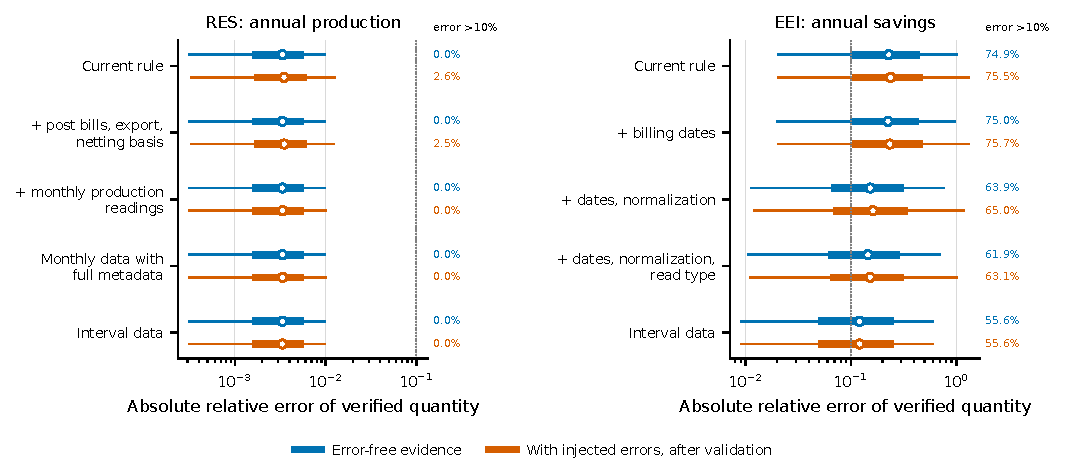
\includegraphics[width=\linewidth]{figures/fig3_error_distributions}
\caption{Synthetic data (attachment Figure 3). Absolute relative error of the verified
quantity by evidence specification: median, interquartile range and 5th--95th
percentile; numbers at right give the share of applicants with error above
\ErrorShareThreshold\%. Blue: error-free evidence; vermilion: with injected errors, after
validation. Error rates are hypothetical.}\label{fig:errors}
\end{figure}

\subsection*{4.3 Which checks need which elements (questions c and d)}

Several results here are true by construction and are stated as logic rather than as
measured performance: a check on bill dates detects a wrong billing period whenever
dates are collected and truthful, and a check on account identifiers detects a second
meter whenever identifiers are collected. The informative results are what happens
\emph{without} those elements, and which statistical screens fail (attachment Table 2 and
Figure 4):

\begin{itemize}
\item Without bill dates, the checks that could still run detected
\DetCurrentEeiPeriod\% (EEI) and \DetCurrentResPeriod\% (RES) of simulated wrong-period
errors (bills from another year, or periods straddling the in-service date).
\item Without account identifiers they detected \DetCurrentEeiDouble\% (EEI) and
\DetCurrentResDouble\% (RES) of cases in which a second meter was included in
pre-installation use. The rule requires a dedicated meter (\S4280.122(a)(16)) but
collects a certification rather than the identifier.
\item A bound on capacity factor from the rated system size and location, which needs no
element beyond those already required, detected the simulated thousand-fold unit errors
in production; it would not detect smaller unit or conversion errors.
\item A plausibility comparison of claimed production with modeled output detected
\DetRulePlausGrossNet\% of cases where exports or bill reductions were reported as
production but only \DetRulePlausNameplate\% of cases where a capacity-times-sun-hours
estimate was reported, at a \StatRuleFpr\% false-positive rate.
\item Two screens did not work. The bill-outlier statistic tested did not detect
transposed digits (area under the ROC curve \AucOutlierTransposed). Comparing claimed
production with the change in utility bills was weak even with exports and the netting
basis known (area \AucBillDiffGrossNet), because facility use changes between years.
Post-installation utility bills for RES projects consequently did not appear on the
accuracy--burden frontier. The simulation did not include fabricated readings, against
which utility records would be the only independent source, so this is not evidence
that such records lack value.
\end{itemize}

\subsection*{4.4 Accuracy and burden together (questions c and d)}

No source reports respondent time by data element for this collection, so the study uses
assumed times, scaled so that the evidence the rule now requires equals
\AnchorResponses{} responses of the notice's average of \AuditHoursPerResponse{} hours.
The scale is arbitrary; relative sizes are more meaningful than minutes. On those
assumptions (Figure~\ref{fig:frontier}), adding bill dates with Agency-side adjustment
adds about \DatesNormBurdenIncreasePct\% to the time for the energy evidence and lowers
the accuracy loss by \DatesNormMareReductionPct\%; the monthly-data specification on the
frontier (\RecElements) adds about \RecBurdenIncreasePct\% and lowers the loss by
\RecMareReductionPct\%. Part of the added time is rework on flagged submissions.

If the applicant uploads the utility's billing-history file instead of typing from
bills, dates, read types and account identifiers arrive with the file at no extra
effort. Whether that is quicker than manual entry depends on how long obtaining the file
takes, which I assumed (\ModeRecUploadBurden{} minutes for the frontier specification,
against \BaseBurden{} for manual entry of the current elements); the Agency could measure
it when testing its portal. Not every utility offers such files or Green Button data
\cite{naesbreq21espi}, so manual entry would have to remain available.

\begin{figure}[!tb]
\centering
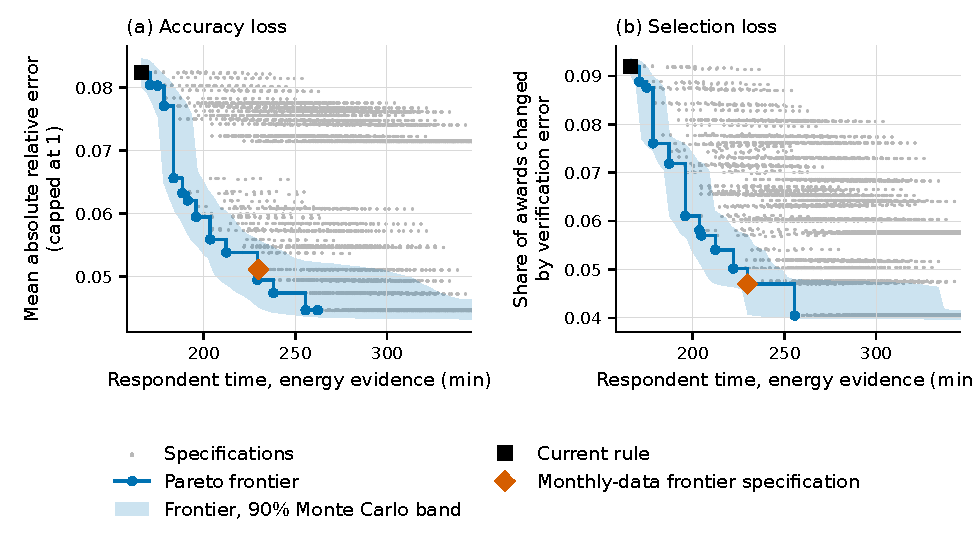
\includegraphics[width=\linewidth]{figures/fig6_frontier}
\caption{Synthetic data, assumed element times (attachment Figure 6). Respondent time and
loss of every feasible combination of \NOptionalElements{} optional elements under manual
entry (gray), the Pareto frontier with a 90\% Monte Carlo band (blue), the current rule
(square) and the monthly-data frontier specification (diamond). (a) Accuracy loss.
(b) Share of awards changed by verification error.}\label{fig:frontier}
\end{figure}

\section*{5. Recommendations}

Table~\ref{tab:recs} ties each recommendation to the PRA question, the provision it
concerns, the evidence in the attachment and the level of validation behind that
evidence. All are within the Agency's authority to design its application instruments
and instructions for this collection and to estimate and certify its burden under
44 U.S.C. 3506(c) and 5 CFR 1320.8 and 1320.9 \cite{cfr1320_8,cfr1320_9}; none requires
amending 7 CFR part 4280.

{\footnotesize
\begin{longtable}{p{0.05\linewidth}p{0.33\linewidth}p{0.2\linewidth}p{0.3\linewidth}}
\caption{Recommendations, provisions and supporting evidence.}\label{tab:recs}\\
\hline
 & Recommendation & Provision and question & Evidence and validation level \\
\hline
\endfirsthead
\hline
 & Recommendation & Provision and question & Evidence and validation level \\
\hline
\endhead
B1 & Reconcile respondents, responses, hours per response and total hours; publish
ratios to sufficient precision & PRA notice, 91 FR 62611; 5 CFR 1320.8(a)(4); question
(b) & Attachment Table 1. Exact arithmetic on published figures (numerical correctness;
observed data) \\
B2 & Correct the respondent description and the request type; identify the docket
document for PRA comments & PRA notice, 91 FR 62610--62611; question (b) & Text of the
notice and docket listing (observed) \\
B3 & Docket the supporting statement and per-instrument burden; state time assumed for
assembling 12+12 months of energy records & 5 CFR 1320.8(a)(4), 1320.3(b)(1);
\S4280.131(b)(17); question (b) & Attachment Table 1 and Section 2.5. Request for
disclosure; the study's element times are hypothetical \\
A1 & State verification method and tolerance for 12-month quantities; assess precision
of EEI savings from 12 bills with historical program data & \S4280.131(b)(17)(i);
definition of Simple Payback, \S4280.104; 5 CFR 1320.8(a)(1), (7); question (a) &
Attachment Figure 3, Tables 3--4 and 8. Verified model of stated assumptions; synthetic
data; request for analysis \\
A2 & Consider collecting monthly production-meter readings with dates & \S4280.131(b)(13),
(b)(17)(i); definition of Annual Energy Production, \S4280.104; question (a) &
Attachment Figure 3, Table 2. Synthetic data; assumes readings supplied are actual
meter readings \\
C1 & Specify bill dates, coded units, read type, account identifier, delivered/net
basis, in-service date, array geometry, affected end-use share as data elements &
\S4280.131(b)(9), (b)(13), (b)(17); \S4280.122(a)(8)(i)(F), (a)(16); 5 CFR 1320.9(d);
question (c) & Attachment Tables 2, 5, 6 and Figure 6. Synthetic data; requirement
traceability from the rule text (observed). Coded units rest on the OIG finding on unit
conversion, not on the simulation. The delivered/net basis is recommended for
interpretability of bills under the metering agreements named in
\S4280.122(a)(8)(i)(F)(3); it did not improve accuracy in the simulation \\
C2 & Publish a machine-readable format (schema and templates) & 5 CFR 1320.9(e), (j);
question (c) & Attachment Section 5 (schema documentation) \\
C3 & Publish the calculation applied to the records (annualization, adjustment,
estimated reads, exports) & Definition of Simple Payback, \S4280.104
(``same input and output conditions''); 5 CFR 1320.9(d); question (c) & OIG audit
finding on calculation guidance (observed); attachment Table 3 (synthetic) \\
D1 & Accept billing-history files and monitoring exports in the application portal &
5 CFR 1320.8(a)(5), 1320.9(j); question (d) & Attachment Table 7. Assumed element
times; the file contains the elements, the time to obtain it is not measured \\
D2 & Validate at entry with deterministic checks; test any statistical screen before
relying on it &
5 CFR 1320.9(j); question (d) & Attachment Table 2, Figure 4. Synthetic data, including
null results \\
D3 & Compute sums, annualized values and payback in the portal & 5 CFR 1320.8(a)(5);
\S4280.131(b)(17); question (d) & OIG audit finding (observed); attachment Table 2
(synthetic) \\
\hline
\end{longtable}
}

Two matters of clarity affect what precision the collected information needs and could
be resolved in the application instructions. The payback tables in \S4280.140(d)(6)
assign points to ``at least 4 and up to 7'' and ``at least 8 and up to 12'' years (EEI)
and ``at least 10 and up to 14'' and ``at least 15 and up to 25'' years (RES), leaving
values between 7 and 8 and between 14 and 15 years unassigned; and the rule does not
say whether twelve billing periods that span more or fewer than 365 days are to be
adjusted. I raise these only as questions about how reported values will be read, not
as comments on the scoring criteria.

\section*{6. Limitations}

\begin{itemize}
\item The applicant-level results are for synthetic applicants. Load shapes for
commercial buildings are State-level aggregates of a modeled building stock;
agricultural load shapes are assumptions and cover electricity only, although many REAP
efficiency projects save propane or diesel; only photovoltaic RES projects are modeled.
\item Error-class rates, noise levels, competition size, funding, non-energy points and
element times are hypothetical. The error rates are not estimates of how often such
errors occur in REAP submissions, and the times attached to data elements are not
measurements. Results that depend directly on them (shares of applicants in error, shares
of awards changed with errors, minutes) are illustrations.
\item Deterministic checks detect the simulated errors they were written for by
construction, and the simulation assumes that a flagged error is corrected and that
requested records are supplied truthfully. Real detection and correction rates would be
lower.
\item The study has no REAP application microdata, and its agreement with real
submissions is not established. The Agency holds historical bills and outcome reports
with which the central question, the precision of twelve-month savings estimates, could
be tested directly; recommendation A1 asks for that.
\item The burden-arithmetic findings in Section 4.1 do not depend on the simulation.
\end{itemize}

\section*{7. Technical attachment}

The attachment (\texttt{attachment\_technical.pdf}) gives the methods, the tables and
figures cited above, the validation rules and the schema element list. The code,
configurations, input provenance and synthetic datasets that reproduce every number in
this comment are in the research repository \texttt{reap-reporting-design},
\url{https://github.com/AvinGupta-ship-it/reap-reporting-design}. The repository is archived
at \url{https://doi.org/10.5281/zenodo.24460622}.

{\footnotesize\setlength{\bibsep}{1pt}
\bibliographystyle{unsrturl}
\bibliography{../paper/references}
}
\end{document}
